\documentclass[english]{article}

\usepackage{babel}
\usepackage{graphicx}
\usepackage{times}
\usepackage{pifont}
\usepackage[margin=1.05in]{geometry}
\usepackage{eurosym}
\usepackage{fancyhdr}
\usepackage[hidelinks]{hyperref}

\pagestyle{fancy}
\fancyhf{}


%HEADER
%**************************************************************************************
\pagestyle{fancy}
\fancyhf{}
%**************************************************************************************
\lhead{Institute of Technology Karlsruhe}		 	 
\rhead{Internship} 
\lfoot{Institute of Data Processing and Electronics}
\cfoot{\thepage}
\rfoot{Alexey Tukalo}
%**************************************************************************************

\date{}
\setlength\parindent{0pt}

\begin{document}

\title{\vspace{2in}Institute of Technology Karlsruhe\\
\small Institute of Data Processing and Electronics\\
\vspace{0.5in}
\includegraphics{savonia.jpg}}

\nopagebreak
\maketitle


\vspace{3in}

\author{
\begin{flushright}
Alexey Tukalo,\\
EFA12SF,\\
Information Technology,\\
Savonia University of Applied Sciences
\end{flushright}
}

\date{\today}
\thispagestyle{empty}

\newpage
\setcounter{page}{1}
\setcounter{tocdepth}{2}
\tableofcontents

\newpage

%MAIN CONTENT ******************************************************************************************************************

\section{Introduction}

I just finished my 4 months internship in Germany at Karlsruhe Institute of Technology. I used to be very excited about the opportunity because: 
\begin{enumerate}
\item The topic fits well my future career prospects.
\item KIT is one of the most respectable researching organisation in Europe.
\item The final product of the research would be able to save many lifes.
\item It is an opportunity to explore industrial culture of the most successful economy in Europe.
\end{enumerate}

The intrenship satisfied my expectations. During the work placement I reached project and personal goals and in result it improved my professional and social skills a lot.


\section{Life}
I want to start my report about my internship in Germany from a story of my trip to Karlsruhe, tips about life in the city and my way back home.

\subsection{Arriving}

I came to Helsinki with my family. In Helsinki I received my German Visa and my parents brought me to the airport there I took a plane to Frankfurt am Main. I choose FinAir's direct plane from Helsinki to Frankfurt.\\

I did not visit Frankfurt this time, because there is a very comfortable bus from the airport directly to the Karlsruhe train station. It is better to order a ticket online for the bus, because the airport is huge and the conformation letter from bus company contains very helpful instructions how to find right bus stop, it is also almost two times cheaper to buy it on the provider's website.\\

An intercity transport system is very messy in Germany, they have a lot of different bus companies and types of trams/trains, but the best option is usually provided by FlixBus. The public transport inside cities is much more consistent. The main option to travel around a cities is trams, it is also possible to use trams for short distance trips outside of cities.\\

Karlsruhe has a hostel right in front of main station, it is the best place to stay, if case of late arriving.

\subsection{Accommodation}

It is a nice idea to have an internship in Karlsruhe in summer, because it is almost impossible to find any kind of short-term accommodation in the middle of semester. The best option is to make sublease for a room with other student who leaves the city for vacation time. It is also possible to get a short-term accommodation in HaDiKo\footnote{The HaDiKo is the biggest self-administered student dormitory in Germany}, but the waiting period is very long. I also want to notice that HaDiKo is very different from a typical Finnish student accommodation. Usually, tenants live in a separate rooms with a tap and shares bathrooms and a kitchen with 12 other guys. \\

It sounds funny, but looking for a good accommodation is Karlsruhe is almost as difficult as looking a good job. Sometimes the market is so crowded by applicants, that flat owners make interviews with future tenants and choose the best one out of 10 or 20 people.\\

KIT is able to help in the search for an accommodation, but their options have 50-70\% higher price than the flats you can find yourself on web. The institute provides several website with advertisements and in my opinion the wg-gesucht.de is the best one in the list. The price is usually broken down in to two peaces: actually price for a property and operational costs. The typical price range is 250-400\euro per month.\\ 

IPE is located in the North Campus of KIT, the campus is far away from city center, it is possible to find a room in a small village near the office, but I wanted to live in the city. So, I traveled to office by a shuttle provided by KIT, the shuttle is going from the South Campus to the North one and vise versa. That's why an accommodation near the South Campus is the best option.\\

In results of the problems in the market, it is typical for students in Karlsruhe to live for a while in hostels, the cheapest option is Kaiser Hostel in the city center, but even cheapest one is much more expensive than normal price for student accommodation. \\

The problems with student accommodation in Germany makes it very popular kind of trap among cheaters, so students have to be extremely careful and never pay rent or deposit before the key are received.\\

\subsection{Food}

The cheapest price for a food is in Lidl and ALDI, there are plenty of them around the city. It is possible to find something specific, for example mussels, in huge EDEKA supermarket, roughly in 500m to the south from University campus. EDEKA also has a network of small shops distributed around the city, but they are a little bit more expensive than ALDI and Lidl.\\

All shops are closed on Sunday and it is a big problem to have an empty fridge on this day. Average food and clothes price is quite close to Finland, but alcohol is much cheaper.\\

Germany has a lot of cheap street food: like kebab, asian noodles, pizza and so on. Normally it is possible to have a lunch at this kind of place for 3-7 \euro. Oxford Cafe is a very popular place among students, it is right in front of South Campus, they have quite low price for meals and drinks, for example it is possible to buy Spaghetti alla Bolognese less than for 4 \euro.\\

The price at North Campus’ canteen is from 3.6 to 6 \euro  for a lunch. The meal is very good there. The menu is based on a traditional German food, it also contains the most famous dishes from other European countries. They are also able to serve the most popular food from other part of the world, but the recipes are changed to fit European taste.

\subsection{Leisure Time}

In my leisure time I used to climb at DAV's climbing center. KIT has a very good gym. It is possible to find a lot of interesting events on meetup.com. An English speaking community of the website held many interesting events for English speaking people, for example they have a Rock and Roll jam every Sunday evening. \\

Summer time, Karlsruhe has a lot of open air activity, for example every weekend they have a free concert behind Karlsruhe Palace. There are many night clubs and bars around the city. Some of them have an entrance fee, other doesn't. Usually the entrance fee and drinks have to be paid only by cash. \\

\subsection{Returning}

I went back to Kuopio through Stuttgart, because SAS offers quite cheap youth tickets from Stuttgart to Denmark and from Copenhagen to Helsinki, so I decided that it is also nice chance to visit Stuttgart. \\

I reached Stuttgart with a FlixBus and I slept one night at the hostel near the train station. Early in a morning I went to the air-port, it is not as big as Fraknfurt's one, so it did not take me much time to catch my plane. From Helsinki to Kuopio I traveled with an OmniBus.

\section{Work Placement}

I worked in the Institute of Data Processing and Electronics, the organisation belongs to the Karlsruhe Institute of Technology. KIT is one of the biggest lab in Europe, they have wide field of topics from nuclear research to medicine and bioengineering.\\

As I already told, IPE placed on the North Campus and it is possible to reach it by KIT Shuttle from the South Campus, a trip takes 20-40 minutes, it depends from traffic. 

\subsection{3D USCT}

I worked in a project called 3D Ultrosound Computer Tomography, shortly USCT. The main goal of the project is development of new image methodology for early breast cancer detection. This type of cancer is one of the most common and dangerous one among women. An early diagnostic of breast cancer significantly increase survival probability of the patient. The USCT team's aim is detection of the tumor with average size small than 5mm.\\

The USCT detector is able to produce three different types of images:

\begin{enumerate}
\item Reflection - contains general structure
\item Sound speed - map of the soundspeed distribution
\item Attenuation - map of the sound wave's amplitude attenuation
\end{enumerate}

The sound speed and attenuation images give doctors an opportunity to classify lesions precisely, while the reflection's one allows them define type of the structure. I worked on fusion of this three different images into the single one, because it makes an analising easier.\\

\subsection{Work organisation}

The most part of time I spent to solve problems assigned to me by supervisor. Once a week USCT has a scrum meeting then people have to tell a short story about a work done at the week and plans for a next one.\\

Every Wednesday morning USCT and Big Data teams have a breakfast together. The breakfast is prepared by one of teammates, randomly chosen by app called Winner Maker. Usually, there is 20 minutes student talk(presentation) in the end of the meeting. Every student has to give the speech in start of his or her work and at the end, before leave the team.\\

Part of my work was out of main area of my supervisors knowledge, so mentor was assigned to me and this task I did in cooperation with the person.

\section{Travels}

I have never been in Germany before and it was very interesting for me to explore the culture, nature and architecture of the country. I was not able to visit every part of Germany for so short period of time and long distance travels around Germany is as expensive as plane from Finland to Germany, so it was pointless to visit really remote cities. That's why I used to be focused on local sites.

\subsection{Transport}

The cheapest way to travel around Germany is buses, but trains have thier own advantages: power sockets, better internet connection, quicker. The difference in price is at least 30-50\%. Germany also has developed network of trams, they are the best option for a short trips\footnote{trips around the areas inside the State}. It is possible to buy day ticket for a tram for 10 \euro, which also allows to travel with any other type of local public transport.

\subsection{Accomodation}

I prefer to travel alone and I don't like to spend time indoor, so I don’t care much about quality of an accommodation, I am trying to find the cheapest one. Usually it is hostels, normal price for hostel in Germany is 15-20\euro for a bed, but sometimes they have an additional price for linens, it can cost guest about 3 \euro. German hostels are a little bit different from hostels in other part of Europe, I visited. It seems to be that Germany is not very popular place for tourists, so the hostels network is not developed, the most part of hostels does not have a proper commune room and kitchen, sometimes they require additional fee for an access to the kitchen. So, probably it is nice idea to look for an accommodation there at AirBnB or CouchSurf it.

\subsection{Cities}
\subsubsection{Karlsruhe}

\begin{figure}
\centerline{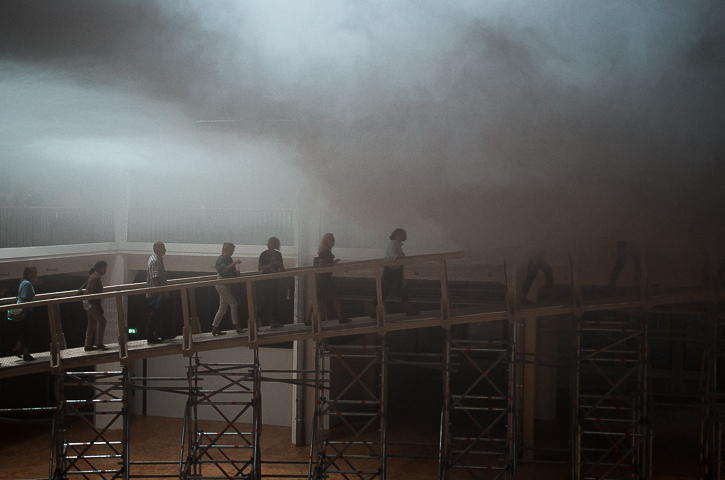
\includegraphics[scale=0.5]{Germany_travel/zkm}}
\caption{ZKM exhibition}
\end{figure}


The city is a quite interesting place, there is a big pedestrian precincts in the city center. The street contains the most part of stores and outlets. It is possible to buy almost any kind of goods here.\\

The main site of the city is Karlsruhe Palace surrounded by a huge park. There are also Botanischer Garten Karlsruhe, Karlsruhe Zoo and many churches. It is possible to find traditional German houses at the west part of Karlsruhe, near Rain.\\

The city has many museums. I was lucky enough to visit the most part of them during the Night of Museums, my favoured one was The State Art Gallery and I did not really like ZKM\footnote{ Centre for Art and Media }. Usually, I am very interested in modern art, but ZKM's exhibition was not as exciting as reviews on TripAdvisor, in my point of view the museums is too empty, maybe they covered part of exhibition for the Night of Museums, but there was nothing to look at.

\begin{figure}
\centerline{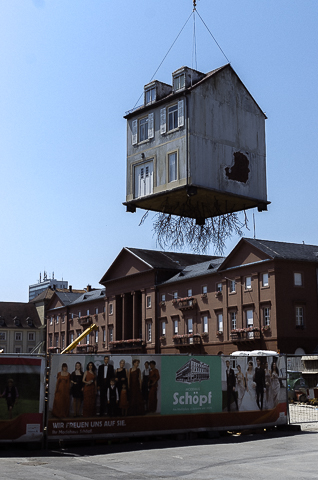
\includegraphics[scale=0.5]{Germany_travel/karlsruhe}}
\caption{The flying house on the streets of Karlsruhe}
\end{figure}

\subsubsection{Frankfurt am Main}
The financial capital of Europe. Two things brought me to the place: the skyscrapers and International Motor Show Germany\footnote{Internationale Automobil-Ausstellung }.\\
\begin{figure}
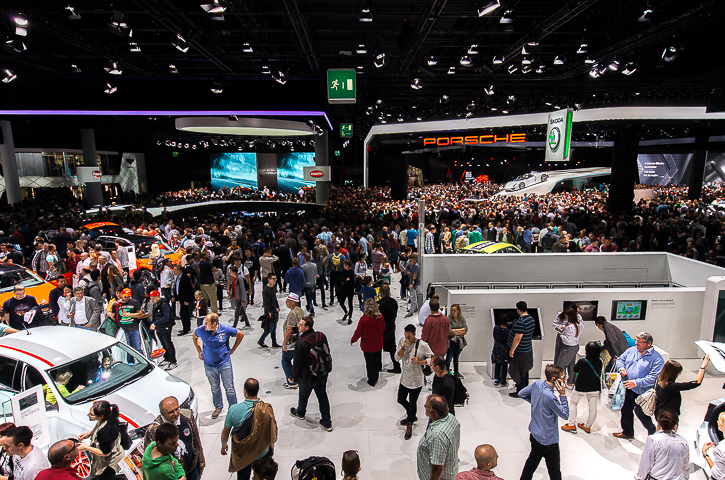
\includegraphics[scale=0.33]{Germany_travel/iaa1}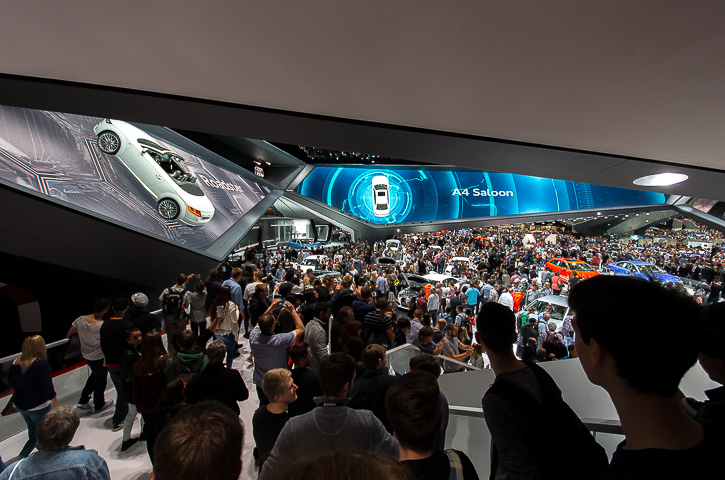
\includegraphics[scale=0.33]{Germany_travel/iaa2}
\caption{International Auto-motor Show}
\end{figure}

The Motor shows is one of the biggest automobile exhibition in the world, the event is hold in Messe Frankfurt once for two years. I wanted to visit IAA since my childhood and finally I have had a chance. The exhibition is very interesting for people related with cars, because it allows to create personal view to the future for the industry and this year my point is different from the point forced by media.\\

Frankfurt is also very famous for the towers, they are not as high as the skyscrapers from USA or asia, but they are impressive for Europe. In addition to the modern buildings, it is possible to find really old streets and squares, which are also nice.\\

\begin{figure}
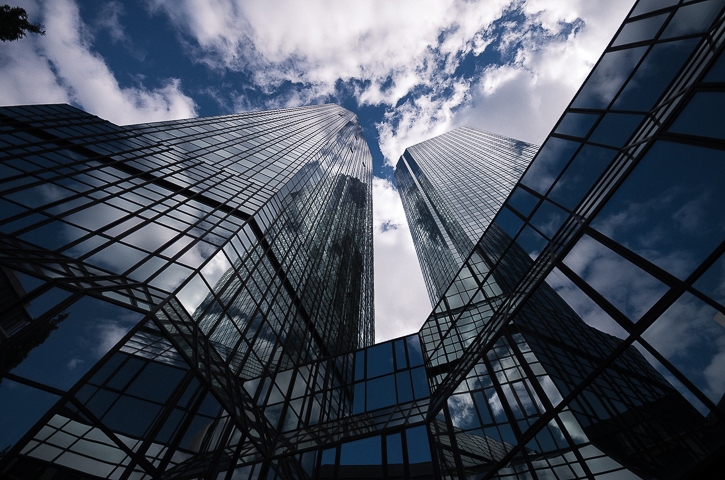
\includegraphics[scale=0.33]{Germany_travel/fk1}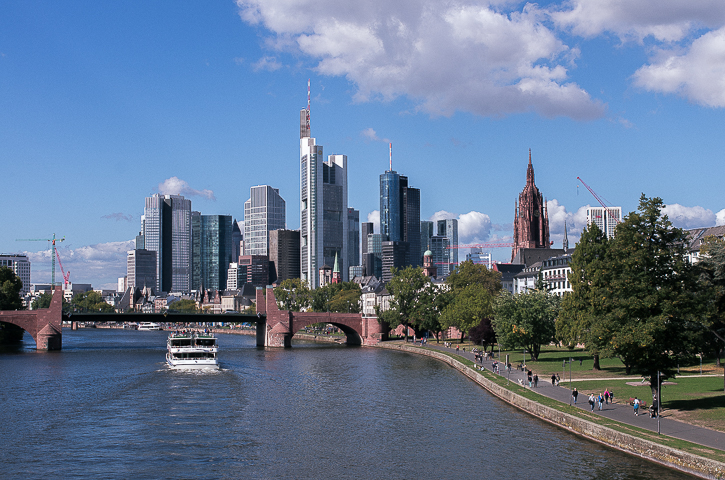
\includegraphics[scale=0.33]{Germany_travel/fk2}\\
\caption{Skyscrapers in Frankfurt}
\end{figure}

Moreover, the city is very famous for the night life, there are a lot of clubs and bars around the city center, but I think that it can be unsafe to hang around the streets at night time, because it is one of the most dangerous city in Germany. I have seen a lot of homeless people, drug dealers and other creepy guys on the streets, especially in the evening and it seems to be that police doesn't care about them at all.\\

In Frankfurt I lived in Frankfurt Central Hostel and to be honest I don't really like the place.

\begin{figure}
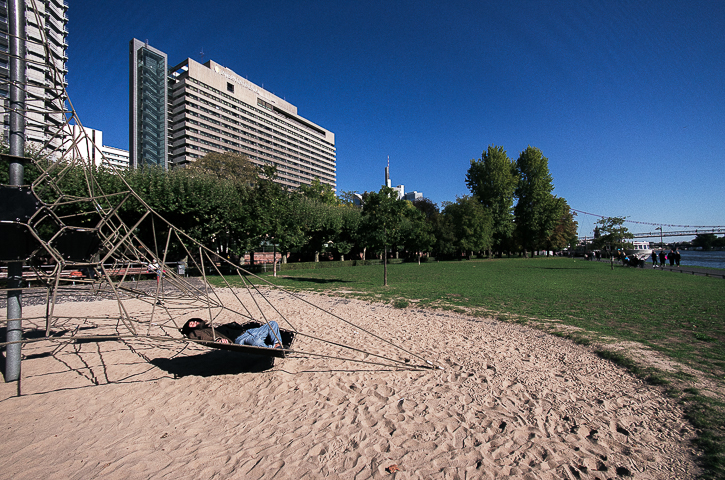
\includegraphics[scale=0.33]{Germany_travel/fk3}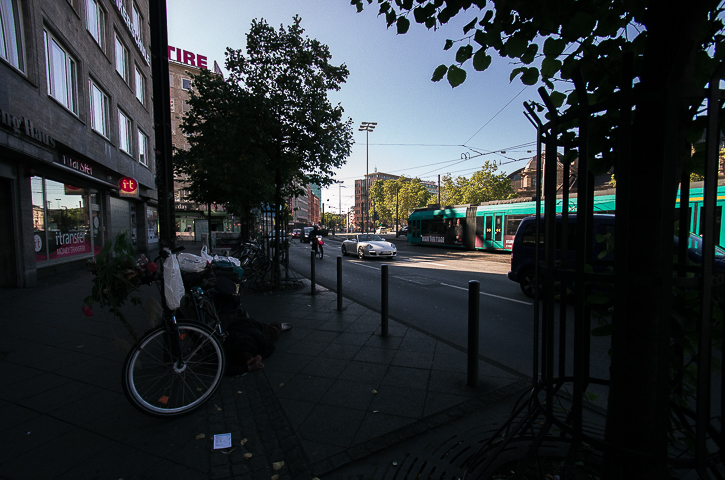
\includegraphics[scale=0.33]{Germany_travel/fk4}\\
\caption{Homeless people in Frankfurt}
\end{figure}

\subsubsection{Baden-Baden}
It is nice small city surrounded by hills. The best way to reach the place from Karlsruhe is tram, it is possible to buy a day ticket for local trams and buses\footnote{about 10 \euro}. I went from Karlsruhe to the train station of Baden-Baden with tram, after that I took bus to the center of the city.\\

Baden-Baden has a quite big car-free area with an old buildings, there are a lot of sites at this place, but I was not interested in them, in my point of view it is simply nice place to hang around.\\

\begin{figure}
\centerline{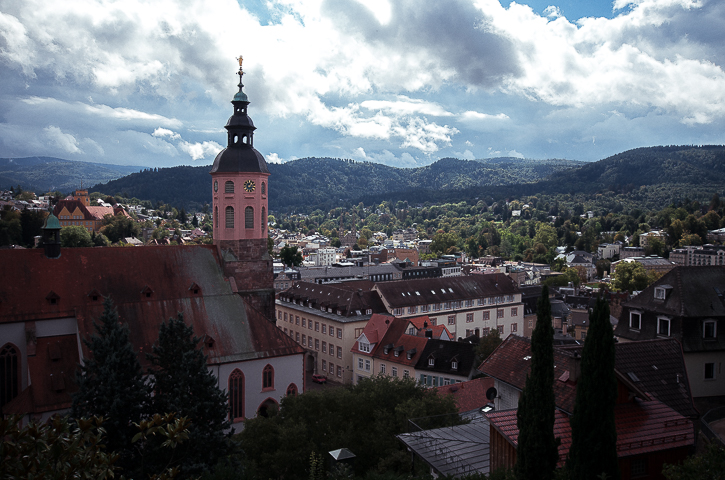
\includegraphics[scale=0.5]{Germany_travel/baden}}
\caption{View to the Baden-Baden from hill}
\end{figure}

The place was especially interesting for me, because it is very famous in Russia, the thermae was very popular among Russian nobility in 18th century. Many famous Russian writers and painters lived in Baden-Baden for a while. 

\subsubsection{Heidenberg}

Heidenberg is one of ten the most attractive for tourists places in entire Germany, because USA wanted to use it as General Headquarters
and in result the city did not suffer from Allied bombing. The city has huge pedestrian precincts with nice Baroque buildings called the Old Town.\\

The main point of tourists interest in Heidenberg is a huge, old and partly broken castle. There is a funicular, which leads to the top of the hill.

\subsubsection{Stuttgart}

Stuttgart is the capital of Baden-Württemberg and the 6th largest city in the Germany. Unfortunately, I can not tell much about the place, because I was only passing there, but I want to visit it again properly in a future.\\

The city is very famous for headquarters of Mercedes and Porsche. The Mercedes logos are almost every there at the place. The city center of Stuttgart is also very beautiful place.

\section{Conclusion}
I am very thankful to Savonia UAS for an opportunity to get this experience in Germany. The internship made me much more confident, allowed me to improve my English, personal and professional skills. This four months brought me a lot of new friends, ideas and impressions. I am very happy to make myself familiar with German way of work, culture and habits. During this time I visited many beautiful places and took hundreds of photos.



\end{document}
